\let\negmedspace\undefined
\let\negthickspace\undefined
\documentclass[journal,12pt,onecolumn]{IEEEtran}
\usepackage{cite}
\usepackage{amsmath,amssymb,amsfonts,amsthm}
\usepackage{algorithmic}
\usepackage{graphicx}
\usepackage{textcomp}
\usepackage{xcolor}
\usepackage{txfonts}
\usepackage{listings}
\usepackage{enumitem}
\usepackage{mathtools}
\usepackage{gensymb}
\usepackage[breaklinks=true]{hyperref}
\usepackage{tkz-euclide} % loads  TikZ and tkz-base
\usepackage{listings}



\newtheorem{theorem}{Theorem}[section]
\newtheorem{problem}{Problem}
\newtheorem{proposition}{Proposition}[section]
\newtheorem{lemma}{Lemma}[section]
\newtheorem{corollary}[theorem]{Corollary}
\newtheorem{example}{Example}[section]
\newtheorem{definition}[problem]{Definition}
%\newtheorem{thm}{Theorem}[section] 
%\newtheorem{defn}[thm]{Definition}
%\newtheorem{algorithm}{Algorithm}[section]
%\newtheorem{cor}{Corollary}
\newcommand{\BEQA}{\begin{eqnarray}}
\newcommand{\EEQA}{\end{eqnarray}}
\newcommand{\define}{\stackrel{\triangle}{=}}
\theoremstyle{remark}
\newtheorem{rem}{Remark}
%\bibliographystyle{ieeetr}
\begin{document}
%
\providecommand{\pr}[1]{\ensuremath{\Pr\left(#1\right)}}
\providecommand{\prt}[2]{\ensuremath{p_{#1}^{\left(#2\right)} }}        % own macro for this question
\providecommand{\qfunc}[1]{\ensuremath{Q\left(#1\right)}}
\providecommand{\sbrak}[1]{\ensuremath{{}\left[#1\right]}}
\providecommand{\lsbrak}[1]{\ensuremath{{}\left[#1\right.}}
\providecommand{\rsbrak}[1]{\ensuremath{{}\left.#1\right]}}
\providecommand{\brak}[1]{\ensuremath{\left(#1\right)}}
\providecommand{\lbrak}[1]{\ensuremath{\left(#1\right.}}
\providecommand{\rbrak}[1]{\ensuremath{\left.#1\right)}}
\providecommand{\cbrak}[1]{\ensuremath{\left\{#1\right\}}}
\providecommand{\lcbrak}[1]{\ensuremath{\left\{#1\right.}}
\providecommand{\rcbrak}[1]{\ensuremath{\left.#1\right\}}}
\newcommand{\sgn}{\mathop{\mathrm{sgn}}}
\providecommand{\abs}[1]{\left\vert#1\right\vert}
\providecommand{\res}[1]{\Res\displaylimits_{#1}} 
\providecommand{\norm}[1]{\left\lVert#1\right\rVert}
%\providecommand{\norm}[1]{\lVert#1\rVert}
\providecommand{\mtx}[1]{\mathbf{#1}}
\providecommand{\mean}[1]{E\left[ #1 \right]}
\providecommand{\cond}[2]{#1\middle|#2}
\providecommand{\fourier}{\overset{\mathcal{F}}{ \rightleftharpoons}}
\newenvironment{amatrix}[1]{%
  \left(\begin{array}{@{}*{#1}{c}|c@{}}
}{%
  \end{array}\right)
}
%\providecommand{\hilbert}{\overset{\mathcal{H}}{ \rightleftharpoons}}
%\providecommand{\system}{\overset{\mathcal{H}}{ \longleftrightarrow}}
	%\newcommand{\solution}[2]{\textbf{Solution:}{#1}}
\newcommand{\solution}{\noindent \textbf{Solution: }}
\newcommand{\cosec}{\,\text{cosec}\,}
\providecommand{\dec}[2]{\ensuremath{\overset{#1}{\underset{#2}{\gtrless}}}}
\newcommand{\myvec}[1]{\ensuremath{\begin{pmatrix}#1\end{pmatrix}}}
\newcommand{\mydet}[1]{\ensuremath{\begin{vmatrix}#1\end{vmatrix}}}
\newcommand{\myaugvec}[2]{\ensuremath{\begin{amatrix}{#1}#2\end{amatrix}}}
\providecommand{\rank}{\text{rank}}
\providecommand{\pr}[1]{\ensuremath{\Pr\left(#1\right)}}
\providecommand{\qfunc}[1]{\ensuremath{Q\left(#1\right)}}
	\newcommand*{\permcomb}[4][0mu]{{{}^{#3}\mkern#1#2_{#4}}}
\newcommand*{\perm}[1][-3mu]{\permcomb[#1]{P}}
\newcommand*{\comb}[1][-1mu]{\permcomb[#1]{C}}
\providecommand{\qfunc}[1]{\ensuremath{Q\left(#1\right)}}
\providecommand{\gauss}[2]{\mathcal{N}\ensuremath{\left(#1,#2\right)}}
\providecommand{\diff}[2]{\ensuremath{\frac{d{#1}}{d{#2}}}}
\providecommand{\myceil}[1]{\left \lceil #1 \right \rceil }
\newcommand\figref{Fig.~\ref}
\newcommand{\systemL}[1]{\stackrel{#1}{\xleftrightarrow{\mathcal{L}}}}
\newcommand{\systemLinv}[1]{\stackrel{#1}{\xleftrightarrow{\mathcal{L}^{-1}}}}


\newcommand\tabref{Table~\ref}
\newcommand{\sinc}{\,\text{sinc}\,}
\newcommand{\rect}{\,\text{rect}\,}
%%
%	%\newcommand{\solution}[2]{\textbf{Solution:}{#1}}
%\newcommand{\solution}{\noindent \textbf{Solution: }}
%\newcommand{\cosec}{\,\text{cosec}\,}
%\numberwithin{equation}{section}
%\numberwithin{equation}{subsection}
%\numberwithin{problem}{section}
%\numberwithin{definition}{section}
%\makeatletter
%\@addtoreset{figure}{problem}
%\makeatother

%\let\StandardTheFigure\thefigure
\let\vec\mathbf


\bibliographystyle{IEEEtran}
\title{ APPENDIX FOR ANALOGOUS SYSTEMS}
\author{EE23BTECH11011- Batchu Ishitha$^{*}$% <-this % stops a space
}
\maketitle




\bigskip

\renewcommand{\thefigure}{\theenumi}
\renewcommand{\thetable}{\theenumi}
%\renewcommand{\theequation}{\theenumi}

Analogous systems of electrical-mechanical systems are like a common language that bridges the gap between electrical and mechanical engineering. They allow us to understand and predict how different components interact, whether they're electrical circuits or mechanical machines. By recognizing similarities between electrical and mechanical elements, engineers can solve problems more efficiently and design better systems. This approach encourages collaboration between specialists from different fields and helps us develop innovative solutions that seamlessly integrate both electrical and mechanical aspects. \\

ELECTRICAL ANALOGIES OF MECHANICAL SYSTEMS:\\

Two systems are said to be analogous if :
\begin{enumerate}
\item The two systems are physically different.
\item Differential equation modelling of these two systems are same.
\end{enumerate} 


There are two types of electrical analogies of translational mechanical systems:
\begin{enumerate}
\item Force-Voltage analogy
\item Force-Current analogy
\end{enumerate} 

FORCE-VOLTAGE ANALOGY:\\
In this, the mathematical equations of translational mechanical system are compared with mesh equations of the electrical system.


\begin{table}[!ht]    
    \centering
     \begin{tabular}{|c|c|} 
    \hline
\textbf{Translational Mechanical System} & \textbf{Electrical System}  \\\hline
    Force(F) & Voltage(V)  \\\hline
    Mass(M) & Inductance (L) \\\hline
    Frictional coefficient(B) & Resistance(R) \\ \hline
    Spring constant(K) & Reciprocal of Capacitance(1/C)  \\\hline
    Displacement(x) & Charge(q) \\ \hline
    Velocity(v) & Current(i)  \\\hline
        \end{tabular}
    
 
      \caption{Input Parameters}
    \label{table:ishitha.g22.nm.54.at1}
\end{table}


Example: 
\begin{figure}[!ht]
    \centering
    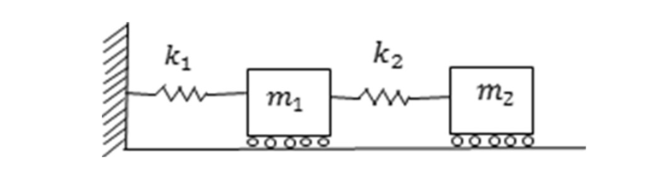
\includegraphics[scale=0.5]{app/figs/g54.fig1.png}
    \caption{ }
    \label{fig:ishitha.g22.nm.54.af1}
\end{figure}  


Equations of translational mechanical system:\\

\begin{figure}[!ht]
    \centering
    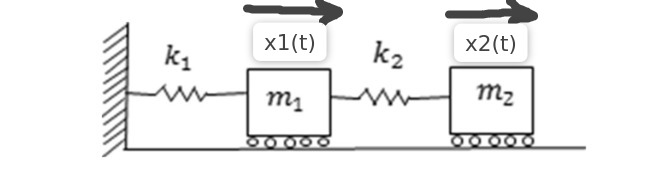
\includegraphics[scale=0.5]{app/figs/g54.fig2.jpeg}
    \caption{ }
    \label{fig:ishitha.g22.nm.54.af2}
\end{figure} 


\begin{align}
m_1\ddot{x_1}(t) - k_2\brak{x_2(t)-x_1(t)}+ k_1x_1(t)&=0
\label{eq:ishitha.g22.nm.54.1.eq}\\
m_2\ddot{x_2}(t) + k_2\brak{x_2(t)-x_1(t)}&=0
\label{eq:ishitha.g22.nm.54.2.eq} 
\end{align}

Mesh equations of electrical system:\\   

\begin{figure}[!ht]
    \centering
    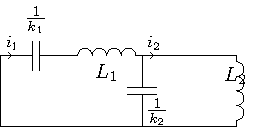
\includegraphics[scale=1.5]{app/figs/tikz.pdf}
    \caption{ }
    \label{fig:ishitha.g22.nm.54.af3}
\end{figure}   
\begin{align}
 k_1\int i_1 \, dt + L_1\frac{di_1}{dt}+k_2\int \brak{i_1-i_2} \, dt &=0\\
 L_2\frac{di_2}{dt}-k_2\int \brak{i_1-i_2} \, dt &=0
\end{align}    

but we know, $i=\frac{dq}{dt}$ 
 \begin{align}
 \implies L_1\ddot q_1 -k_2\brak{q_2-q_1} + k_1q_1  &=0 \\
 \implies L_2\ddot q_2+k_2\brak{q_2-q_1} \, dt &=0
\end{align}  

FORCE-CURRENT ANALOGY:\\
In this , the mathematical equations of the translational mechanical system are compared with the nodal equations of the electrical system.


\begin{table}[!ht]    
    \centering
     \begin{tabular}{|c|c|} 
    \hline
\textbf{Translational Mechanical System} & \textbf{Electrical System}  \\\hline
    Force(F) &Current(i) \\\hline
    Mass(M) & Capacitance(C) \\\hline
    Frictional coefficient(B) &Reciprocal of Resistance(1/R) \\ \hline
    Spring constant(K) & Reciprocal of Inductance(1/L)  \\\hline
    Displacement(x) & Magnetic Flux($\psi $)\\ \hline
    Velocity(v) &  Voltage(V) \\\hline
        \end{tabular}
    
 
    \label{table:ishitha.g22.nm.54.at2}
\end{table}

